% !TEX option = -shell-escape
\documentclass[UTF8,a4paper]{ctexart}
\usepackage{hyperref,float,graphicx,fancyhdr}
\usepackage[cache=false]{minted}

\pagestyle{fancy}
%\thispagestyle {fancy}
\renewcommand{\sectionmark}[1]{\markboth{\thesection.\ #1}{}}
\lhead{\bfseries \leftmark}

\chead{}
\rhead{}
\lfoot{qhy}
\cfoot{\url{https://github.com/285571052}}
\rfoot{\thepage}
\setlength{\headheight}{13pt}
\renewcommand{\headrulewidth}{0.4pt}
\renewcommand{\footrulewidth}{0.4pt}

\setminted{breaklines,breakanywhere,linenos,frame=single}
\newminted{tex}{breaklines,breakanywhere,linenos,frame=single}

\author{qhy}
\date{\today}
\title{笔记}
\begin{document}
    \maketitle
    \tableofcontents
    \newpage

    \section[Latex]{Latex \footnote{\url{https://en.wikibooks.org/wiki/LaTeX}}}
        \subsection{下划线}
        对花括号内的内容产生下划线,其中$\sim$表示空格
        \begin{texcode}
\underline{~~}
        \end{texcode}

        \subsection[页面样式和页码]{页面样式和页码 \footnote{\url{http://latexfly.com/docs/packages/fancyhdr.html}}}
        \begin{texcode}
\usepackage{fancyhdr}

\pagestyle{fancy}
%\thispagestyle {fancy}
\renewcommand{\sectionmark}[1]{\markboth{\thesection.\ #1}{}}
\lhead{\bfseries \leftmark}

\chead{}
\rhead{}
\lfoot{qhy}
\cfoot{\url{https://github.com/285571052}}
\rfoot{\thepage}
\setlength{\headheight}{13pt}
\renewcommand{\headrulewidth}{0.4pt}
\renewcommand{\footrulewidth}{0.4pt}

\setminted{breaklines,breakanywhere,linenos,frame=single}
\newminted{tex}{breaklines,breakanywhere,linenos,frame=single}
        \end{texcode}


        \subsection{各种标题}
        \begin{texcode}
\chapter
\section
\subsection
\subsubsection
\paragraph
\subparagraph
        \end{texcode}

        \subsection[脚注]{脚注 }
            \subsubsection{一般用法}
            \begin{texcode}
\footnote{This is footnote.}
            \end{texcode}

            \subsubsection[在标题中使用脚注,但脚注不在目录中显示]
            {在标题中使用脚注,但脚注不在目录中显示
             \footnote{\url{https://liam0205.me/2013/08/26/LaTeX-Footnote-In-Section-Title/}}}
             \begin{texcode}
 \documentclass{article}
 \begin{document}
 \tableofcontents
 \section[Section Title]{Section Title\footnote{This is footnote.}}
 \end{document}
             \end{texcode}

        \subsection{超链接}
        \begin{texcode}
\usepackage{hyperref}
\url{https://github.com/285571052}
        \end{texcode}
        \subsection{插入图片}
        \begin{minted}{tex}
\usepackage{float,graphicx}
% float 和 H是把图片放在当前位置,不浮动
\begin{figure}[H]
    \centering
    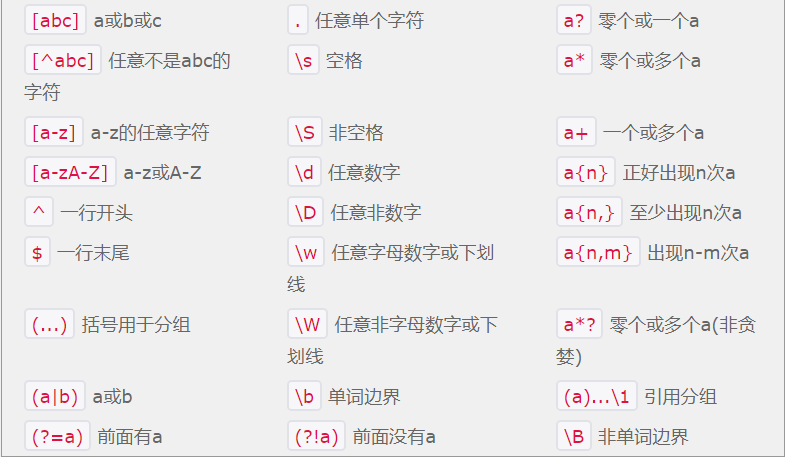
\includegraphics[scale=0.5]{assets/note_f547c.png}
    % scale是缩放比例
    \caption{正则表达式语法}
    \label{fig-20170729110818}
\end{figure}

        \end{minted}

        \subsection[代码粘贴、着色]{代码粘贴、着色 \footnote{\url{https://github.com/gpoore/minted}}}

        \subsubsection{配置}
        \begin{itemize}
                    \item [1. ] 安装 atom-latextool 而不是 atom-latex
                    \item [2. ] python 安装 Pygments
                    \item [3. ] 在.tex文件中加入\mintinline{tex}{% !TEX option = -shell-escape}
        \end{itemize}

        \subsubsection{使用方法}
        \begin{texcode}
\usepackage[cache=false]{minted}
%全局设置 , 其中{C++}可以省略
\setminted{c++}{breaklines,breakanywhere,linenos,frame=single}
\begin{minted}[breaklines,breakanywhere,linenos,frame=single]{latex}
...
\end{minted}

\mint{tex}{%new line code}

\mintinline{%inline code}
        \end{texcode}

            \subsubsection{shortcuts}
            上一章节不能直接显示对应环境的end代码,即上一章节的代码并不能直接放在 minted的环境下,解决办法是采用shortcuts
            \begin{texcode}
\newminted{cpp}{gobble=2,linenos}
\begin{cppcode}
template <typename T>
    T id(T value) {
    return value;
}
\end{cppcode}
            \end{texcode}
            \subsubsection{支持的语言}
            \begin{minted}{bat}
pygmentize -L lexers
            \end{minted}


    \section{Windows 批处理}
        \subsection{help 命令}
        有关某个命令的详细信息,请键入 HELP 命令名

        e.g. 查看start命令的详细信息
        \begin{minted}{bat}
help start
        \end{minted}

        \subsection{start 命令}
        启动一个单独的窗口以运行指定的程序或命令。

        e.g. 等待程序运行结束
        \begin{minted}{bat}
start /w notepad.exe
        \end{minted}

        \subsection{逐行读取文本}
        \begin{minted}{bat}
For /F %%a in (iprange.conf) Do (
	set flg=
	findstr /B %%a finish.txt >nul 2>&1 && set flg=1
	if not defined flg (
		echo %%a > tmprange.conf
		start /w gscan_quic_windows_amd64.exe -iprange=tmprange.conf
		echo "%date:~0,4%-%date:~5,2%-%date:~8,2%:%%a finish" >> logging.txt
		echo %%a >> finish.txt
	)else echo "%date:~0,4%-%date:~5,2%-%date:~8,2%:%%a skip" >> logging.txt
)
        \end{minted}

    \section{正则表达式}
        \subsection{语法}
        \begin{figure}[H]
            \centering
            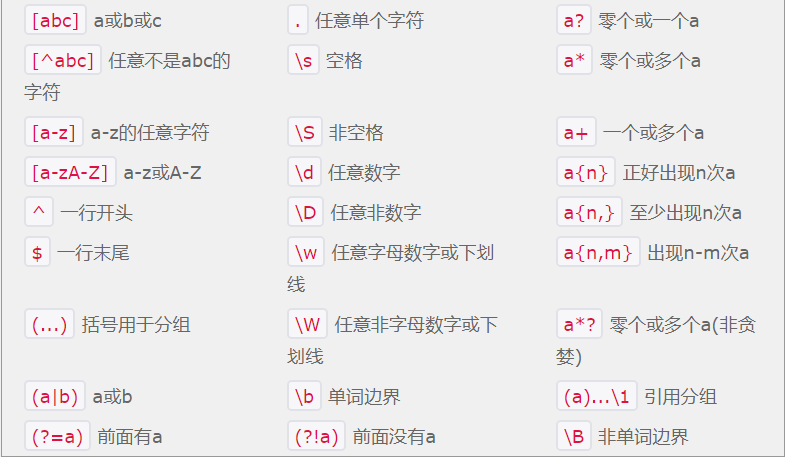
\includegraphics[scale=0.5]{assets/note_f547c.png}
            \caption{正则表达式语法}
            \label{fig-20170729110818}
        \end{figure}

    \section{atom}
        \subsection[鼠标单击、双击打开文件细节区别]{鼠标单击、双击打开文件细节区别 \footnote{http://blog.csdn.net/zsl10/article/details/52021274}}

        ATOM自版本1.6开始优化了打开文件方式。

        场景如下:

        有时候开发人员需要点击查看大量的文件,此时如果打开了多个固定标签(tab),那么编辑器将显得非常混乱,ATOM自版本1.6起引入了临时标签的概念,即当每次在项目树菜单下,鼠标单击打开文件时,将在一个临时标签页打开该文件。

        双击打开文件:鼠标双击打开文件即我们经常使用的打开文件方式,每次都建立一个固定标签来打开文件。

        单、双击打开文件方式配置:atom$\to$ file $\to$ setting$\to$core$\to$ Allow Pending Pane Items

    \section{Shell}
        \subsection[分割生成的文件按规律命名并添加扩展名]{分割生成的文件按规律命名并添加扩展名\footnote{\url{https://seofangfa.com/shell/shell-split.html}}}
        \begin{minted}{shell}
split -l 5 -a 5 -d iprange.conf iprange-
ls|grep iprange-|xargs -n1 -i mv {} {}.conf
        \end{minted}

    \section{Others}
    \subsection[rss 订阅特定 bilibili 的 up 主]{rss 订阅特定 bilibili 的 up 主 \footnote{https://www.v2ex.com/t/315041}}

    使用 \textbf{Google Apps Script},把mid后面的参数替换掉即可。

    \begin{texcode}
https://script.google.com/macros/s/AKfycbyUWJda1KGh6v-_p35CW5qGeT6IWSPUiK8oFzteuBnm6fNh88c/exec?mid=221648

https://space.bilibili.com/221648#!/
    \end{texcode}

    \subsection[加速任何Android智能手机的小窍门]{加速任何Android智能手机的小窍门 \footnote{\url{https://youtu.be/e5k1-_jOLPM}}}

    打开开发者模式$\to$ 设置 $\to$ 开发者选项 $\to$ 窗口动画缩放/过渡动画缩放/动画程序时长缩放 $\to$ 关闭

        \subsection[解锁pdf文件]{解锁pdf文件 \footnote{
\url{
http://zh.wikihow.com/%E8%A7%A3%E9%94%81%E5%8A%A0%E5%AF%86%E7%9A%84PDF%E6%96%87%E4%BB%B6
}}}
        把pdf文件上传到GoogleDrive$\to$在GoogleDrive中打开对应的pdf文件$\to$打印到本地

        \subsection{中国电信在线投诉}
        有啥问题打电话不能解决就到这里填单吧。

        地址:\url{http://61.129.250.80/workorder-web/189_menhu.jsp}

        \subsection{newifi 开启SSH}
        以下网页替换成自己路由器的ip,打开网页即可使用SSH连接路由器。

        \url{http://192.168.99.1/newifi/ifiwen_hss.html}

\end{document}
